% The index relabelling behind transverse contraction, after ITransverse.jl (Fig. 3).
% The dictionary between the two labellings is left to the caption; this is a small inline figure.
%
% Standalone: compiles to imgs/rotation.pdf.
% Inline:     with \usepackage{standalone}, % The index relabelling behind transverse contraction, after ITransverse.jl (Fig. 3).
% The dictionary between the two labellings is left to the caption; this is a small inline figure.
%
% Standalone: compiles to imgs/rotation.pdf.
% Inline:     with \usepackage{standalone}, % The index relabelling behind transverse contraction, after ITransverse.jl (Fig. 3).
% The dictionary between the two labellings is left to the caption; this is a small inline figure.
%
% Standalone: compiles to imgs/rotation.pdf.
% Inline:     with \usepackage{standalone}, % The index relabelling behind transverse contraction, after ITransverse.jl (Fig. 3).
% The dictionary between the two labellings is left to the caption; this is a small inline figure.
%
% Standalone: compiles to imgs/rotation.pdf.
% Inline:     with \usepackage{standalone}, \input{imgs/rotation}.
\documentclass[tikz,border=2pt]{standalone}
\usepackage{amsmath,amssymb}
\usetikzlibrary{arrows.meta}

\definecolor{tnbulk}{RGB}{86,196,229}
\definecolor{tntemp}{RGB}{244,162,97}

\begin{document}
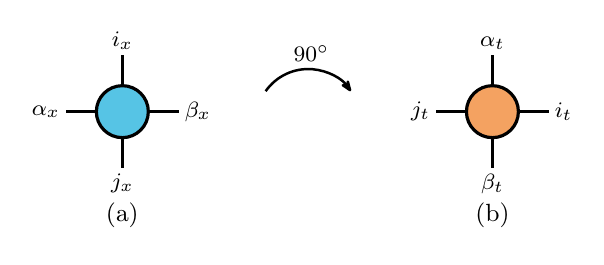
\begin{tikzpicture}[
    >={Stealth[round,length=2.0mm]},
    leg/.style={draw=black, line width=1.15pt},
    Wx/.style={circle, draw=black, fill=tnbulk, line width=1.15pt, minimum size=6.6mm, inner sep=0pt},
    Wt/.style={circle, draw=black, fill=tntemp, line width=1.15pt, minimum size=6.6mm, inner sep=0pt},
    tag/.style={font=\small},
    idx/.style={font=\footnotesize, inner sep=1.5pt},
  ]

  \def\L{0.72}

  % (a) the spatial tensor
  \node[Wx] (A) at (0,0) {};
  \draw[leg] (A) -- ++(0,\L)  node[idx, above] {$i_x$};
  \draw[leg] (A) -- ++(0,-\L) node[idx, below] {$j_x$};
  \draw[leg] (A) -- ++(-\L,0) node[idx, left]  {$\alpha_x$};
  \draw[leg] (A) -- ++(\L,0)  node[idx, right] {$\beta_x$};
  \node[tag] at (0,-1.32) {(a)};

  % the rotation
  \draw[->, line width=0.9pt] (1.82,0.26) arc[start angle=145, end angle=35, radius=0.66];
  \node[idx, anchor=south] at (2.4,0.58) {$90^\circ$};

  % (b) the same tensor read along time
  \node[Wt] (B) at (4.7,0) {};
  \draw[leg] (B) -- ++(0,\L)  node[idx, above] {$\alpha_t$};
  \draw[leg] (B) -- ++(0,-\L) node[idx, below] {$\beta_t$};
  \draw[leg] (B) -- ++(-\L,0) node[idx, left]  {$j_t$};
  \draw[leg] (B) -- ++(\L,0)  node[idx, right] {$i_t$};
  \node[tag] at (4.7,-1.32) {(b)};

\end{tikzpicture}
\end{document}
.
\documentclass[tikz,border=2pt]{standalone}
\usepackage{amsmath,amssymb}
\usetikzlibrary{arrows.meta}

\definecolor{tnbulk}{RGB}{86,196,229}
\definecolor{tntemp}{RGB}{244,162,97}

\begin{document}
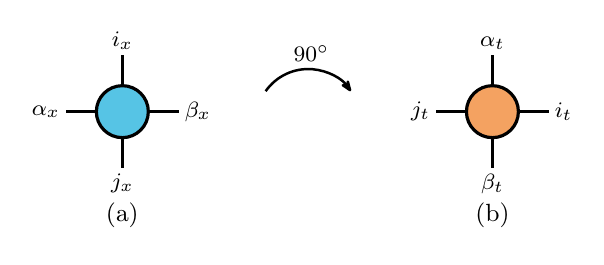
\begin{tikzpicture}[
    >={Stealth[round,length=2.0mm]},
    leg/.style={draw=black, line width=1.15pt},
    Wx/.style={circle, draw=black, fill=tnbulk, line width=1.15pt, minimum size=6.6mm, inner sep=0pt},
    Wt/.style={circle, draw=black, fill=tntemp, line width=1.15pt, minimum size=6.6mm, inner sep=0pt},
    tag/.style={font=\small},
    idx/.style={font=\footnotesize, inner sep=1.5pt},
  ]

  \def\L{0.72}

  % (a) the spatial tensor
  \node[Wx] (A) at (0,0) {};
  \draw[leg] (A) -- ++(0,\L)  node[idx, above] {$i_x$};
  \draw[leg] (A) -- ++(0,-\L) node[idx, below] {$j_x$};
  \draw[leg] (A) -- ++(-\L,0) node[idx, left]  {$\alpha_x$};
  \draw[leg] (A) -- ++(\L,0)  node[idx, right] {$\beta_x$};
  \node[tag] at (0,-1.32) {(a)};

  % the rotation
  \draw[->, line width=0.9pt] (1.82,0.26) arc[start angle=145, end angle=35, radius=0.66];
  \node[idx, anchor=south] at (2.4,0.58) {$90^\circ$};

  % (b) the same tensor read along time
  \node[Wt] (B) at (4.7,0) {};
  \draw[leg] (B) -- ++(0,\L)  node[idx, above] {$\alpha_t$};
  \draw[leg] (B) -- ++(0,-\L) node[idx, below] {$\beta_t$};
  \draw[leg] (B) -- ++(-\L,0) node[idx, left]  {$j_t$};
  \draw[leg] (B) -- ++(\L,0)  node[idx, right] {$i_t$};
  \node[tag] at (4.7,-1.32) {(b)};

\end{tikzpicture}
\end{document}
.
\documentclass[tikz,border=2pt]{standalone}
\usepackage{amsmath,amssymb}
\usetikzlibrary{arrows.meta}

\definecolor{tnbulk}{RGB}{86,196,229}
\definecolor{tntemp}{RGB}{244,162,97}

\begin{document}
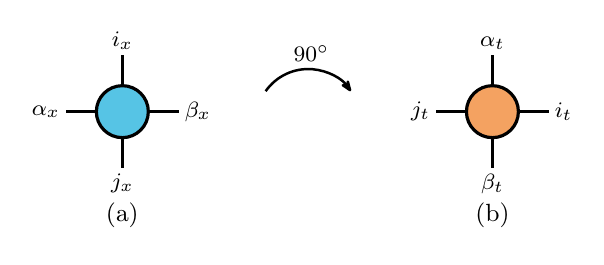
\begin{tikzpicture}[
    >={Stealth[round,length=2.0mm]},
    leg/.style={draw=black, line width=1.15pt},
    Wx/.style={circle, draw=black, fill=tnbulk, line width=1.15pt, minimum size=6.6mm, inner sep=0pt},
    Wt/.style={circle, draw=black, fill=tntemp, line width=1.15pt, minimum size=6.6mm, inner sep=0pt},
    tag/.style={font=\small},
    idx/.style={font=\footnotesize, inner sep=1.5pt},
  ]

  \def\L{0.72}

  % (a) the spatial tensor
  \node[Wx] (A) at (0,0) {};
  \draw[leg] (A) -- ++(0,\L)  node[idx, above] {$i_x$};
  \draw[leg] (A) -- ++(0,-\L) node[idx, below] {$j_x$};
  \draw[leg] (A) -- ++(-\L,0) node[idx, left]  {$\alpha_x$};
  \draw[leg] (A) -- ++(\L,0)  node[idx, right] {$\beta_x$};
  \node[tag] at (0,-1.32) {(a)};

  % the rotation
  \draw[->, line width=0.9pt] (1.82,0.26) arc[start angle=145, end angle=35, radius=0.66];
  \node[idx, anchor=south] at (2.4,0.58) {$90^\circ$};

  % (b) the same tensor read along time
  \node[Wt] (B) at (4.7,0) {};
  \draw[leg] (B) -- ++(0,\L)  node[idx, above] {$\alpha_t$};
  \draw[leg] (B) -- ++(0,-\L) node[idx, below] {$\beta_t$};
  \draw[leg] (B) -- ++(-\L,0) node[idx, left]  {$j_t$};
  \draw[leg] (B) -- ++(\L,0)  node[idx, right] {$i_t$};
  \node[tag] at (4.7,-1.32) {(b)};

\end{tikzpicture}
\end{document}
.
\documentclass[tikz,border=2pt]{standalone}
\usepackage{amsmath,amssymb}
\usetikzlibrary{arrows.meta}

\definecolor{tnbulk}{RGB}{86,196,229}
\definecolor{tntemp}{RGB}{244,162,97}

\begin{document}
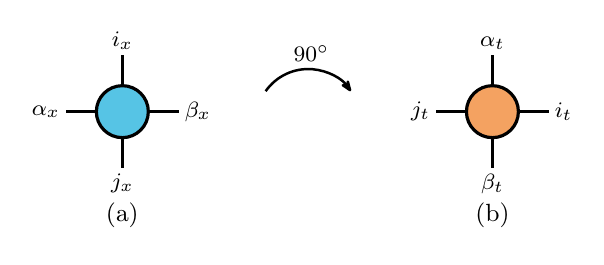
\begin{tikzpicture}[
    >={Stealth[round,length=2.0mm]},
    leg/.style={draw=black, line width=1.15pt},
    Wx/.style={circle, draw=black, fill=tnbulk, line width=1.15pt, minimum size=6.6mm, inner sep=0pt},
    Wt/.style={circle, draw=black, fill=tntemp, line width=1.15pt, minimum size=6.6mm, inner sep=0pt},
    tag/.style={font=\small},
    idx/.style={font=\footnotesize, inner sep=1.5pt},
  ]

  \def\L{0.72}

  % (a) the spatial tensor
  \node[Wx] (A) at (0,0) {};
  \draw[leg] (A) -- ++(0,\L)  node[idx, above] {$i_x$};
  \draw[leg] (A) -- ++(0,-\L) node[idx, below] {$j_x$};
  \draw[leg] (A) -- ++(-\L,0) node[idx, left]  {$\alpha_x$};
  \draw[leg] (A) -- ++(\L,0)  node[idx, right] {$\beta_x$};
  \node[tag] at (0,-1.32) {(a)};

  % the rotation
  \draw[->, line width=0.9pt] (1.82,0.26) arc[start angle=145, end angle=35, radius=0.66];
  \node[idx, anchor=south] at (2.4,0.58) {$90^\circ$};

  % (b) the same tensor read along time
  \node[Wt] (B) at (4.7,0) {};
  \draw[leg] (B) -- ++(0,\L)  node[idx, above] {$\alpha_t$};
  \draw[leg] (B) -- ++(0,-\L) node[idx, below] {$\beta_t$};
  \draw[leg] (B) -- ++(-\L,0) node[idx, left]  {$j_t$};
  \draw[leg] (B) -- ++(\L,0)  node[idx, right] {$i_t$};
  \node[tag] at (4.7,-1.32) {(b)};

\end{tikzpicture}
\end{document}
